\documentclass[twoside,twocolumn]{article}
\renewcommand\thesection{\roman{section}} 
\renewcommand\thesubsection{\Alph{subsection}}
\usepackage{amsmath}
\usepackage{amssymb}
\usepackage[english]{babel}
\usepackage{graphicx}
\usepackage{titlesec}
\usepackage{indentfirst}
\setlength{\parindent}{2em}
\usepackage[hmarginratio=1:1,top=32mm,columnsep=20pt]{geometry}
\titleformat{\section}[block]{\large\scshape\centering}{\thesection.}{1em}{} % Change the look of the section titles
\titleformat{\subsection}[block]{\large}{\thesubsection.}{1em}{} % Change the look of the section titles
\title{Power Consumption and Delay}
\author{}  % no author
\begin{document}
\maketitle
%\clearpage
\section{Introduction}
\section{Related Work}
\section{SYSTEM MODEL AND PROBLEM FORMULATION}
In this section,we give an overview of our approach toward balanced delay and power consumption. As shown in figure 1,the system architecture that we consider comprises : a set of Roadside Units(RSUs),a set of fog devices and a set of cloud servers.The RSUs receive requests from users and send them to a set N of fog devices through a Local Area Network(LAN),which act as users' interfaces. Fog nodes can process some delay-sensitive,light-level requests and forward other delay-tolerant requests to a set N of cloud servers through a Wide Area Network(WAN). Each cloud server hosts a lot of homogeneous computing machines.Since the WAN covers a large geographical area from the fog to the cloud, the transmission delay can not be omitted[compared to the LAN].The communication delay and the bandwidth limitation should be taken into account. Moreover,the computation delay of fog node or cloud node also should be considered. Hence,we mainly consider consumption and delay in three components(i.e.,fog layer,WAN transmission,cloud layer). The used notation is summarized in table I.
\begin{figure}[h]
\centering
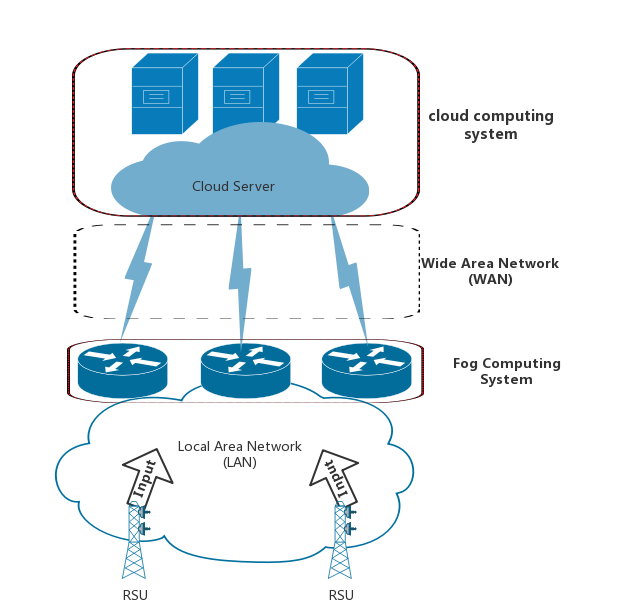
\includegraphics[scale=0.3]{3.png}
\caption{Overall architecture of a fog-cloud computing system}
\label{fig:label}
\end{figure}

\begin{table}[h]
	\centering
	\begin{tabular}{p{1cm}p{6cm}}
	\hline
	Symbol & Definition \\\hline
	$i,N,\mathcal{N}$ & index, number, set of fog devices\\
	$j,M,\mathcal{M}$ & index, number, set of cloud devices\\
	$l_i$             & traffic arrival rate to fog device $i$\\
	$x_i$             & workload assigned to fog device $i$\\
	$\lambda_{ij}$    & traffic rate dispatched from fog device $i$ to cloud server $j$\\
	$y_j$             & workload assigned to cloud server $j$\\
	$L$               & total input from all RSUs\\
	$X$               & workload allocated for fog computing\\
	$Y$               & workload allocated for cloud server\\
	$P$               & power consumption\\
	$D$               & delay\\
	$v_i$             & service rate for fog device $i$\\
	$f_j$             & machine CPU frequency at cloud server $j$\\
	$\sigma_j$        & on/off state of cloud server $j$\\
	$n_j$             & machine number in cloud server $j$\\
	$d_{i,j}$         & communication delay from fog device $i$ to cloud server $j$\\\hline
	\end{tabular}
	\caption{Symbols}
\end{table}


\subsection{System Model}

\textit{1) Power Consumption of Fog Device:} The computation power consumption of fog device \textit{i} can be calculated by a function of the computation amount $X_i$.The function must be a monotonic increasing and strictly convex function. The piece-wise linear function and quadratic function are two candidates. Generally speaking, the power consumption functions of the fog computing device have a number of different forms as long as the functions satisfy the following constraints: \textit{a):}  the function result always increases as the computation amount increases. \textit{b):} the marginal power consumption for each fog device is increasing.For simplicity but without loss of generality,the power consumption $p_i^{fog} $ of device $i$ is defined as follows.
$$ p_i^{fog} \triangleq a_ix_i^2+b_ix_i+c_i $$
where $x_i$ is the computation amount and $a_i,b_i,c_i$ are non-negative,pre-determined parameters. 

\textit{2) Communication Delay of Fog Device:} We assume that it is a queueing system for the fog device to process requests. For the device $i$ with traffic arrival rate $x_i$ and service rate $v_i$, the computation delay $D_i^{fog}$ which includes waiting time and service time is 
$$ D_i^{fog} \triangleq \frac{1}{v_i-x_i} .$$

\textit{3) Power Consumption of Cloud Server:} As mentioned before, each cloud server hosts numerous homogeneous computing machines. We simply assume that the CPU frequencies of these machines are equal in a cloud server. The number of turned-on machines in cloud server $j$ is denoted by $n_j$ In this situation, the power consumption of cloud server $j$ can be expressed as the product of the turned-on machine consumption value and the number of machines in server $j$. We approximate the power consumption value of each machine in server $j$ by a function of CPU frequency $f_j$:$P^{mh} = A_jf_j^p+B_j$, where $A_j$ and $B_j$ are positive constants, and $p$ is in the range of 2.5 to 3. 

At a specific moment, some cloud servers are powered on for computation service whereas more server are powered off for energy saving especially when the workload decreased. We use a binary variable $\sigma_j$ denote the on/off state of cloud server $j$. Specifically, 0 indicates that the server is off and 1 means on. Hence, the power consumption $P_j^{cloud}$ of the cloud server $j$ can be calculated by multiplying the number of turned-on machines and each machine power consumption value.
$$P_j^{cloud} = \sigma_jn_j\left(A_jf_j^p+B_j\right)$$

\textit{4) Communication Delay of Cloud Server:} The delay of cloud server can be obtained by $D_i^{cloud} = t_{queue}+t_{service}$. We model the system as a queueing network, and the cloud can be modeled as $M/M/n$ queue. According to queueing theory, average queueing time $t_{queue}$ is $\frac{C(n,\lambda/\mu)}{n\mu-\lambda}$,where n is the number of turned-on machines,$\lambda$ and $\mu$ respectively indicate traffic arrival rate and service rate. We assume each machine in cloud server $j$ has the same service rate $\mu_{j}$. Thus, the $\mu_j$ can be converted to $f_j/K$,where k is average cycles per request.(cycles/request). According to the definition of service rate, the service time $t_{service}$ is the reciprocal of service rate $\mu$. Thus, the total computation delay of cloud server is given by
$$D_j^{cloud} \triangleq \sigma_j\left[\frac{C\left(n_j,y_jK/f_j\right)}{n_jf_j/K-y_j} + \frac{K}{f_j}\right].$$

\textit{5) Communication delay of dispatch:} We use $d_{ij}$ to record the transmission delay from fog device $i$ to the cloud server $j$. Let the binary variable $\lambda_{ij}$ denote the traffic rate dispatched from the fog device $i$ to the cloud server $j$. The communication delay of dispatch is 
$$ D_{ij}^{com} \triangleq d_{ij}\lambda_{ij} .$$

\subsection{Constraints}

\textit{1) Fog Device Limitation:} For the fog device $i$, the processing ability is limited due to the physical constraint. There exists an maximum computing capability $x_i^{max}$. Obviously, the workload $x_i$ assigned to the fog device $i$ is no more than the maximum $x_i^{max}$ and the arrival rate $l_i$. In summary, we have

\begin{equation}
0 \leq x_i \leq min\left\{x_i^{max} , l_i\right\} \qquad \forall  i\in \mathcal{N}.
\end{equation}


\textit{2) Cloud Server Limitation:} For the cloud server j , We have 
\begin{equation}
y_j \geq 0 \qquad \forall i \in \mathcal{M}.
\end{equation}
For each machine in cloud server j, $f_j^{max}$ denotes the max CPU frequency of the machine and $f_j^{min}$ denotes the minimum. Then we have 
\begin{equation}
f_j^{min} \leq f_j \leq f_j^{max} \qquad \forall j \in \mathcal{M}.
\end{equation}

In addition, the number of machines in cloud server $j$ is an integer which is no more than the upper bound $n_j^{max}$. Then we have
\begin{equation}
n_j \in \left\{ 0,1,2,\dots,n_j^{max} \right\} \qquad \forall j \in \mathcal{M}
\end{equation}
At last, $\sigma_j$ should be a binary variable.
\begin{equation}
\sigma_j \in \left\{0,1\right\} \qquad \forall j \in \mathcal{M}
\end{equation}

\textit{3) Workload Constraint:} Assuming that L denote the total requests input from all RSUs. These requests should be sent to a N set of fog devices. Thus, it satisfies 
$$
L \triangleq \sum_{i \in \mathcal{N}} l_i
$$

Let $\mathit{X}$,$\mathit{Y}$ respectively denote the workload for fog computing and cloud computing. Then we have
$$
\left\{
\begin{array}{lr}
\mathit{X} \triangleq \sum_{i \in \mathcal{N}} x_i &  \\
\mathit{Y} \triangleq \sum_{j \in \mathcal{M}} y_j. &
\end{array}
\right.
$$

The requests from RSUs can be devided into two parts, which are processed by fog devices or cloud servers,respectively. To be more specific, the corresponding relationship is as following.

Workload balance constraint for each cloud server
\begin{equation}
\sum_{i \in \mathcal{N}} \lambda_{ij} = y_j \qquad \forall j \in \mathcal{M}
\end{equation}

Workload balance constraint for each fog device
\begin{equation}
l_i - x_i = \sum_{j \in \mathcal{M}} \lambda_{ij} \qquad \forall i \in \mathcal{M}
\end{equation}
Obviously , from (6)(7) we can obtain 
\begin{equation}
L = X+Y
\end{equation}

\textit{4)WAN Bandwidth Constraint:} For the transmission path from fog device $i$ to the fog server $j$, let $\lambda_{ij}^{max}$ denotes the max bandwidth capacity. Moreover, these transmission paths do not overlap with each other. The constraint of WAN communication bandwidth is as follows:
\begin{equation}
0 \leq \lambda_{ij} \leq \lambda_{ij}^{max} \qquad \forall i \in \mathcal{N}; \quad \forall j \in \mathcal{M}
\end{equation}
\subsection{Problem Formulation}
We propose our model toward trade-off on power consumption and delay in vehicular fog computing system. we want to minimize the power consumption ,meanwhile ensuring the low-delay	The vehicular end experienced delay consist of the computation delay and transmission delay.
The total delay of the proposal model is defined as 
$$
D^{sys} \triangleq \sum_{i \in \mathcal{N}} D_i^{fog} + \sum_{j \in \mathcal{M}} D_j^{cloud} + \sum_{i \in \mathcal{N}}\sum_{j \in \mathcal{M}} D_{ij}^{com}.
$$

The power consumption consists of the fog layer and the cloud layer, which is shown as below.
$$
P^{sys} \triangleq \sum_{i \in \mathcal{N}} p_i^{fog} + \sum_{j \in \mathcal{M}} p_j^{fog}.
$$

We consider the problem of minimizing the power consumption ,as mentioned before, while guaranteeing the max tolerance delay $\overline{D}$ for vehicular end. Then we have the PP
\begin{equation*}
\begin{split}
%
\min_{x_i,y_j,\lambda_{ij},f_j,n_j,\omega_j} p^{sys}  \\  
s.t.\left\{
\begin{array}{lr}
D^{sys} \leq \overline{D} &  \\
(1)-(8). &
\end{array}
\right.
%	
\end{split}
\end{equation*}


The exact solution of the above problem consists in solving the above problem as  a mixed integer non-linear
programming (MINLP) problem, which is a NP-Hard problem. Thus, in case of large scale applications, the problem solving time is unacceptable.

\end{document}
